\subsection{Aufbau des Programms}
Das Programm ist in 3 funktionale Teile gegliedert. Dazu zählt das Einlesen der Audiodateien, die benötigte Signalverarbeitung inklusiver Berechnung der gewünschten Parameter und das Speichern der gewonnenen Werte in Form einer Excel-Datei. Die einzelnen Module werden in der Datei $main.m$ zusammengeführt. Außerdem werden da die gewünschten Einstellungen überprüft und entsprechende Parameter an die verschiedenen Funktionen weitergegeben.
\paragraph{Einlesen der Audiodaten}
Die Audiodateien liegen im WAV-Format als Stereoaufnahme vor. Zunächst wird eine Liste mit allen Dateien in einem bestimmten Ordner erstellt, damit die Dateien nacheinander eingelesen werden können. Im nächsten Schritt werden die beiden Kanäle voneinander getrennt, um diese dann in die Signalverarbeitung zu übergeben.
\paragraph{Signalverarbeitung}
Das Kernstück der Signalverarbeitung ist eine periodische Korrelationsfunktion, die den linken und rechten Kanal miteinander korreliert. Die dabei entstandene Korrelationsfunktion wird dann weiter untersucht. Als nächstes wird eine Art Einhüllende berechnet, die ein Maß für die Steilheit der Kurve ist. Wie bereits im Abschnitt 3.2 beschrieben, wird dann mit Hilfe der Methode der kleinsten Quadrate eine Glockenkurve so angepasst, dass sie den Verlauf der Hüllkurve der KKF möglichst gut abbildet. Die Parameter ripple, $\sigma$, Gleichanteil und Zeitverschiebung des Maximums aus dem Ursprung werden danach an eine Funktion übergeben, die diese Daten in einer Excel-Tabelle speichert.
Der Signalverarbeitungsteil hat auch die Möglichkeit aus einer Datei verschieden viele Abschnitte mit unterschiedlichen Längen zu korrelieren. Damit kann man aus relativ wenigen aufgenommen Signalen relativ viele Signal-Abschnitte gewinnen, die der Korrelation zugeführt werden.
\paragraph{Speicherung}
Die Speicherung der Daten erfolgt in einer Excel-Datei. Nach jedem Korrelationsdurchgang werden die berechneten Werte einer Matrix hinzugefügt. Dabei wird zu erst der Dateiname des Samples und alles dazugehörigen Werte gespeichert. Desweiteren wird die Zeitdauer des Ausschnitts, sowie die Sampling-Rate gespeichert.

\begin{figure}[ht!]
  \centering
  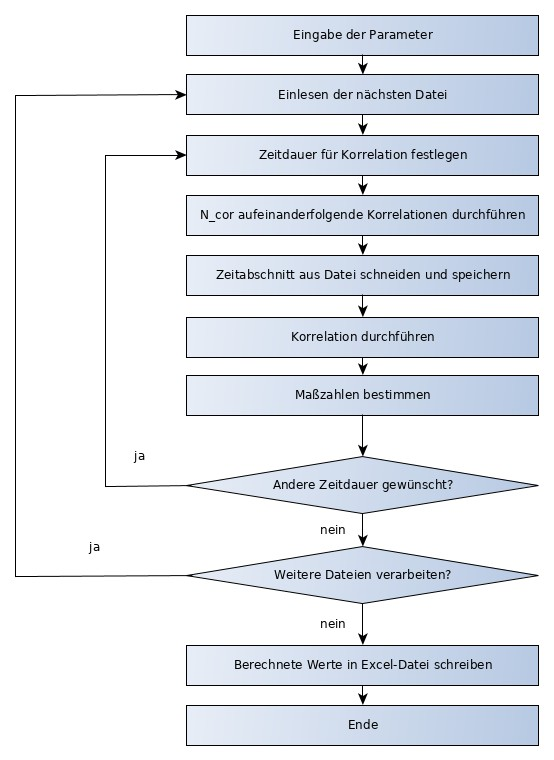
\includegraphics[scale=0.6]{img/pap}
  \caption{Programmablaufplan}
  \label{figure1}
\end{figure}

\subsection{Beispielparameter}
Im Folgenden betrachten wir einige Zeilen Code, die verdeutlichen sollen, welche Möglichkeiten man zur Einstellung hat.
\begin{lstlisting}
path = 'RECORDS\lucas';
excel_path = 'RESULTS\data.xlsx';
% results (display/save_param/save_all)
output = 'display';

% calculate correlation with (xcorr/freqMult)
calc = 'freqMult';

% plot in (samples/seconds)
x_axes = 'seconds';

% set priority (time/length)
priority = 'time';

% start of correlation in audio file in seconds
% time -> and durations 
t_start = 8;
t_dur = [0.5 2];

% amount of correlations 
Ncor_init = [4 1];

% length -> length of correlation in samples
Lcor = 8192; 
\end{lstlisting}
In \textbf{Zeile 1 und Zeile 2} werden die Ein und Ausgabepfade definiert. Dabei spielt es für die Variable $path$ keine Rolle, ob es sich um einen Ordner oder eine Datei handelt. Dies wird automatisch erkannt und im Programm entsprechend berücksichtigt.\newline
In \textbf{Zeile 4} kann man einstellen, wie die Ergebnisse präsentiert werden. Die Option \textit{display} zeigt die enstehenden Graphen auf dem Bildschirm an. Nur bei geringer Anzahl an Korrelationen zu empfehlen, da der Rechenaufwand sehr groß ist. \textit{save$\_$param} sorgt dafür, dass alle Parameter in einer Excel-Tabelle gespeichert werden, ohne dass man die Möglichkeit hat, sich die Graphen dazu anzuschauen. Die letzte Möglichkeit ist die Option \textit{save$\_$all}, welche dazu dient, die Diagramme zusätzlich zu der Exceldatei abzuspeichern.\newline
In \textbf{Zeile 7} wird angegeben, welche Methode zur Berechnung verwendet wird. \textit{xcorr} ist hierbei die Korrelation im Zeitbereich und benutzt die Octave-Funtkion xcorr, welche zero padding betreibt. Nutzt man die Option \textit{freqMult} wird das Ergebnis im Frequenzbereich berechnet, ohne dass es zu zero padding kommt. Die Berechnung im Frequenzbereich ist bei großen Blocklängen zu empfehlen, da es wesentlich schneller ist.\newline
In \textbf{Zeile 10} kann eingestellt werden, ob die x-Achse der Diagramme in Sekunden oder Samples skaliert wird. Je nach Anwendungsfall zu entscheiden.\newline
\textbf{Zeile 13} gibt an, ob die folgenden Zeiteinstellungen oder die angegebene Blocklänge zu korrelieren ist. \textit{time} ist hierbei offensichtlich die Priorisierung der Zeitangaben, während \textit{length} die Blocklänge bevorzugt.\newline
\textbf{Zeile 17} gibt an ab wann die Verarbeitung starten soll. Im Beispiel wird alles was vor Sekunde 8 kommt, vernachlässigt. \newline
In \textbf{Zeile 18} wird ein Array deklariert, welches Zeitdauern enthält. In diesem Beispiel werden Zeitdauern von 0.5 und 2 Sekunden benutzt. \newline
\textbf{Zeile 21} gibt nun in Verbindung mit \textbf{Zeile 18} an, wie oft die jeweilige Zeitdauer nacheinander korreliert werden soll. In unserem Beispiel heißt das, dass 4 hintereinanderliegende Blöcke mit einer Länge von 0.5 Sekunden verarbeitet werden und danach ein Block mit einer Länge von 2 Sekunden. Das Array welches durch N$\_$cor definiert wird, muss immer genauso groß sein, wie das Array t$\_$dur.\newline
\textbf{Zeile 24} gibt an wie lang die Blocklänge für die Korrelation sein soll. Wird nur mit der Option \textit{length} der priority-Einstellung verwendet. Wird die Berechnung im Frequenzbereich durchgeführt, ist es sinnvoll, 2-er Potenzen zu benutzen, da die FFT nur mit Blocklängen umgehen kann, die eine Potenz von 2 sind. Ist dies nicht der Fall, wird der Rest der Werte mit 0 aufgefüllt.\newline

\subsection{Erweiterung der Analysemöglichkeiten}
Um das Octave-Script um weitere Analysemethoden zu erweitern, ist vor allem die Funktion $analysis$ interessant, die die folgende Signatur hat:
\begin{lstlisting}
function [ripple, sigma, ex, area, lagDiff, timeDiff, envelope, reg_gauss, 
                sorted, reg_exp] = analysis(correlation, lags, rate, x_axes)
\end{lstlisting}
Es gibt 4 Eingabeparameter. \textbf{correlation} ist ein Zeilenvektor, welcher die Werte der diskreten Korrelation enthält. \textbf{x$\_$axes} ist ein String und die restlichen Parameter sind normale Zahlenwerte. Alle zu berechnenden Maßzahlen werden dem Aufrufer der Funktion zurückgegeben. Um sinnvolle Plots erstellen zu können, werden unter anderem die Hüllkurve und die sortierten Werte zurückgegeben.  
Innerhalb der Funktion $analysis$ werden nun einige Funktionen zur eigentlichen Analyse der Daten aufgerufen. Dazu zählen die Funktionen $calc\_ripple$, $calc\_reg$ und $calc\_envelope$. Sollen weitere Maßzahlen berechnet werden, müssen hier neue Funktionen hinzugefügt werden. Außerdem müssen die Funktionen $buildXLSMatrix$ und $writeExcel$ erweitert werden, damit die entsprechenden Kennwerte auch entsprechend abgespeichert werden.
\subsection{Probleme} 
Zu Beginn unserer Arbeit wurde die Korrelation zuerst in Python implementiert. Allerdings nahm die Berechnungsdauer mit zunehmende Blocklänge stark zu. Da die .wav Dateien mit 44100Hz abgetastet werden werden die zu berechnenden Summen schnell sehr groß. Wie in der Theorie und im Abschnitt zur Software schon erklärt, wird nun Octave und die Fouriertransformation genutzt. \\\\Darauf aufbauend war noch die Problemstellung der Bemessung der korrelierten Signale zu lösen. Dabei mussten Maßzahlen entstehen, die viele verschiedene Faktoren beachteten und möglichst gute Aussagen über ,,Peakyness'' und Streuung der KKF trafen. Die Idee war einen Fit mit einer Funktion wie der Gauß-Kurve, die als Parameter schon eine Verteilung beinhaltet. Allerdings ist die KKF nach der Berechnung sehr ,,eckig'' und weißt viele Nullstellen auf. Um den Fit nicht durch diese Eigenschaften verzerren zu lassen, wird die KKF durch einen Tiefpass gefiltert. Auf die geglättete Kurve angewendet, ist die angewendete Regression aussagekräftiger.
